\documentclass[]{article}

\usepackage{graphicx}
\usepackage{float}
\usepackage[a4paper,top=2.5cm,bottom=2.5cm,left=2.5cm,right=2cm]{geometry}
\usepackage{subcaption}
\usepackage[table,xcdraw]{xcolor}
\usepackage{makecell}
\usepackage{tabularx}
\usepackage{enumitem}

\setlength{\tabcolsep}{13pt}
\renewcommand{\arraystretch}{2.3}


\begin{document}
	\pagenumbering{gobble}
	
	\begin{figure}[H]
		\centering
		
\includegraphics[scale=0.29]{FrontPage.png}
	\end{figure}
	

	\newpage
	\pagenumbering{arabic}	


	\tableofcontents
	
	\newpage
	
	
	\section{Introduction}
	
	\subsection{Purpose}
	The purpose of this document is defining the main design principles of the CLup software system, taking as input the concepts defined in the RASD. This document treats many topics regarding the software design. It starts from the high-level architecture choices and continues with the description of the main components, also describing how they interact with each other. The last section is about the system implementation, integration and the testing phases, useful to the developer to put together the various design aspects during the system development. 
	\\The reader can find a more detailed list of the treated topics in section 1.3.6.
	
	
	\subsection{Scope}
	
	\begin{paragraph}
		\newline
		CLup is an application that aims to provide the users with the possibility to queue to enter in a store, preserving as much as possible their safety and health. The lining up procedure can be done in two different ways: nearby the store with a physical ticket or from the application, where a virtual ticket is generated. In this way the crowd in the neighborhood of the stores is reduced, and so as a consequence the risks to get in touch with other people is decreased too. People lining up from home will start approach the store only when the system provides them a notification. Customers will then enter the store only when their turn has come, by the recognition of the QRcode on their ticket.\\
		This application is built in order to be as easy as possible so that it can be used by customers of all the ages. Customers can simply line-up to the store they prefer, but they can also take advance of other services that are implemented inside the book a visit feature. Store managers have a different interface to deal with the system, as they have different things to check and for sure different goals, such as monitor entrances/exits and then allow more people in the store if it is possible. \\
		However, more specific and deep descriptions of the available features can be found in the RASD document.\\
		
	\end{paragraph}

	\subsection{Definitions, Acronyms, Abbreviations}
	
		In this section we explain the meaning of some technical terms used in the document.
		
		
		\subsubsection{Definitions}
		
			\medskip
			
			\begin{tabular}{|c|l|}
				\hline
				\rowcolor[HTML]{DCDCDC} 
				\textbf{QR CODE} & \makecell[l]{A \textit{Quick Response code} is a kind of bar-code, readable by machines to retrieve \\information} \\ \hline
				\textbf{prova} & \makecell[l]{prova} \\ \hline
				\rowcolor[HTML]{DCDCDC} 
				\textbf{prova2} & \makecell[l]{prova} \\ \hline
			\end{tabular}
		
		
		\subsubsection{Acronyms}
		
			\medskip
			
			\begin{tabular}{|c|l|}
				\hline
				\rowcolor[HTML]{DCDCDC} 
				\textbf{RASD} & \makecell[l]{A \textit{Quick Response code} is a kind of bar-code, readable by machines to retrieve information} \\ \hline
				\textbf{DD} & \makecell[l]{Design Document} \\ \hline
				\rowcolor[HTML]{DCDCDC} 
				\textbf{GPS}& \makecell[l]{Global Positioning System} \\ \hline
			\end{tabular}
		
		
		\subsubsection{Abbreviations}
						
			
		\subsubsection{Revision History}
		
		
		\subsubsection{Reference Documents}
		
		
		\subsubsection{Document Structure}
		
			Here a list of the topics treated in each chapter of this Design Document.
			
			\paragraph{Chapter 1} is an introductory chapter, where are presented the purpose and the scope of this document. It also includes tables about acronyms and technical definitions.	
			
			\paragraph{Chapter 2} is the core of the Design Document. Here we can find the main architectural decisions, starting from the high-level design patterns. Then, there's a description of every single components and the interaction with each other. Lots of diagrams are included among the different subsections to better explain the presented concepts.
			
			\paragraph{Chapter 3} presents a deep description of the User Interface by means of a large number of detailed mockups and UX diagrams.
			
			\paragraph{Chapter 4} contains the strongest link to the RASD. In fact, it shows a mapping between the requirements presented in the RASD and the architectural components presented in chapter 2.
			
			\paragraph{Chapters 5} aims to give to the developers the guidelines of the implementation, integration and test phases, from both an high-level and a low-level point of view.
		
			\paragraph{Chapters 6 and 7} contains respectively tables about the effort spent by each group member in writing this document and the document references.
			\newpage
			
		
		\section{Architectural Design}
			
			\subsection{Overview}
				\begin{paragraph}
					\newline
					Three logic layers define the architecture of the application. This division has been made so that eventual needed updates that are related to only one of the parts does not affect the other two, leaving them independent from this point of view. The application has to be made in the Client-Server behavior, where the clients can join from different devices and work on the system through some hardware and software components that will be better explained into details in the next sections of the document. The three discussed layers are:\\
					\begin{itemize}
						\item Presentation Level (P) : it’s the higher level of the application and deals directly with the users. It shows to the users the actions they can do in a specific moment and so it has to display them the info in a well-ordered and understandable way. All the features and functions need to be made properly available when needed\\
						\item Business Logic or Application Layer (A) :  it’s the intermediate level the application and so it handles the data between the other two layers, checking and elaborating them so that the logic and the functionalities of the application are preserved and handled in the right way.\\
						\item Data Access Layer (D) : It’s the level that assures to keep data independent to the logic of the application. It handles the info with respect to the databases of the system, managing them when requested by the layer on its top.\\ \newline
					\end{itemize}
					
					
					Ideally, the sequence of the process begins with the request of the user to do a specific action when he wants to apply for a displayed available functionality, and to do this he will set the activation of a specific method that will trigger the application logic to manage it.
When the user concludes his procedure to being inserted in the queue of a store, sends a request to the server that handles the received data: if the lining-up has been made from home then the virtual ticket (its data) will be sent to the user, otherwise If the request of the ticket has been made from the totem at the store, the data sent back from the server will contain a valid or not valid ticket (the logic takes care of how many physical tickets have already been released and stops  sending valid tickets if the threshold has been reached yet).\\
					\newline
What’s more, for what concerns the users, every time they select and submit their preferences (mean of transport, favorite products, …) they will send data to the server, which makes them stored in the databases and allows the user to proceed through the next steps of the lining up procedure. Stored data will be useful when the user requests to see his statistics: they will be elaborated and sent back to the user, that would see them displayed on the screen of his device.\\
					\newline
The system has to deal with store managers too, and so the server will periodically update the available data of the manager, that would monitor the situation of the store in real time: this will allow the manager to send the request to allow more people enter the store, handled by the application logic and whose results are displayed back to the manager.

				
				\end {paragraph}
				
				
	
	\newpage
	\textbf{} \\
	\textbf{Visit subsystem}
	\medskip \newline
	The visit subsystem aims to handle everything that is related to booking visits. It is composed by 4 components as the reader can see in the picture below. 
	\newline
	\begin{figure}[H]
		\centering
		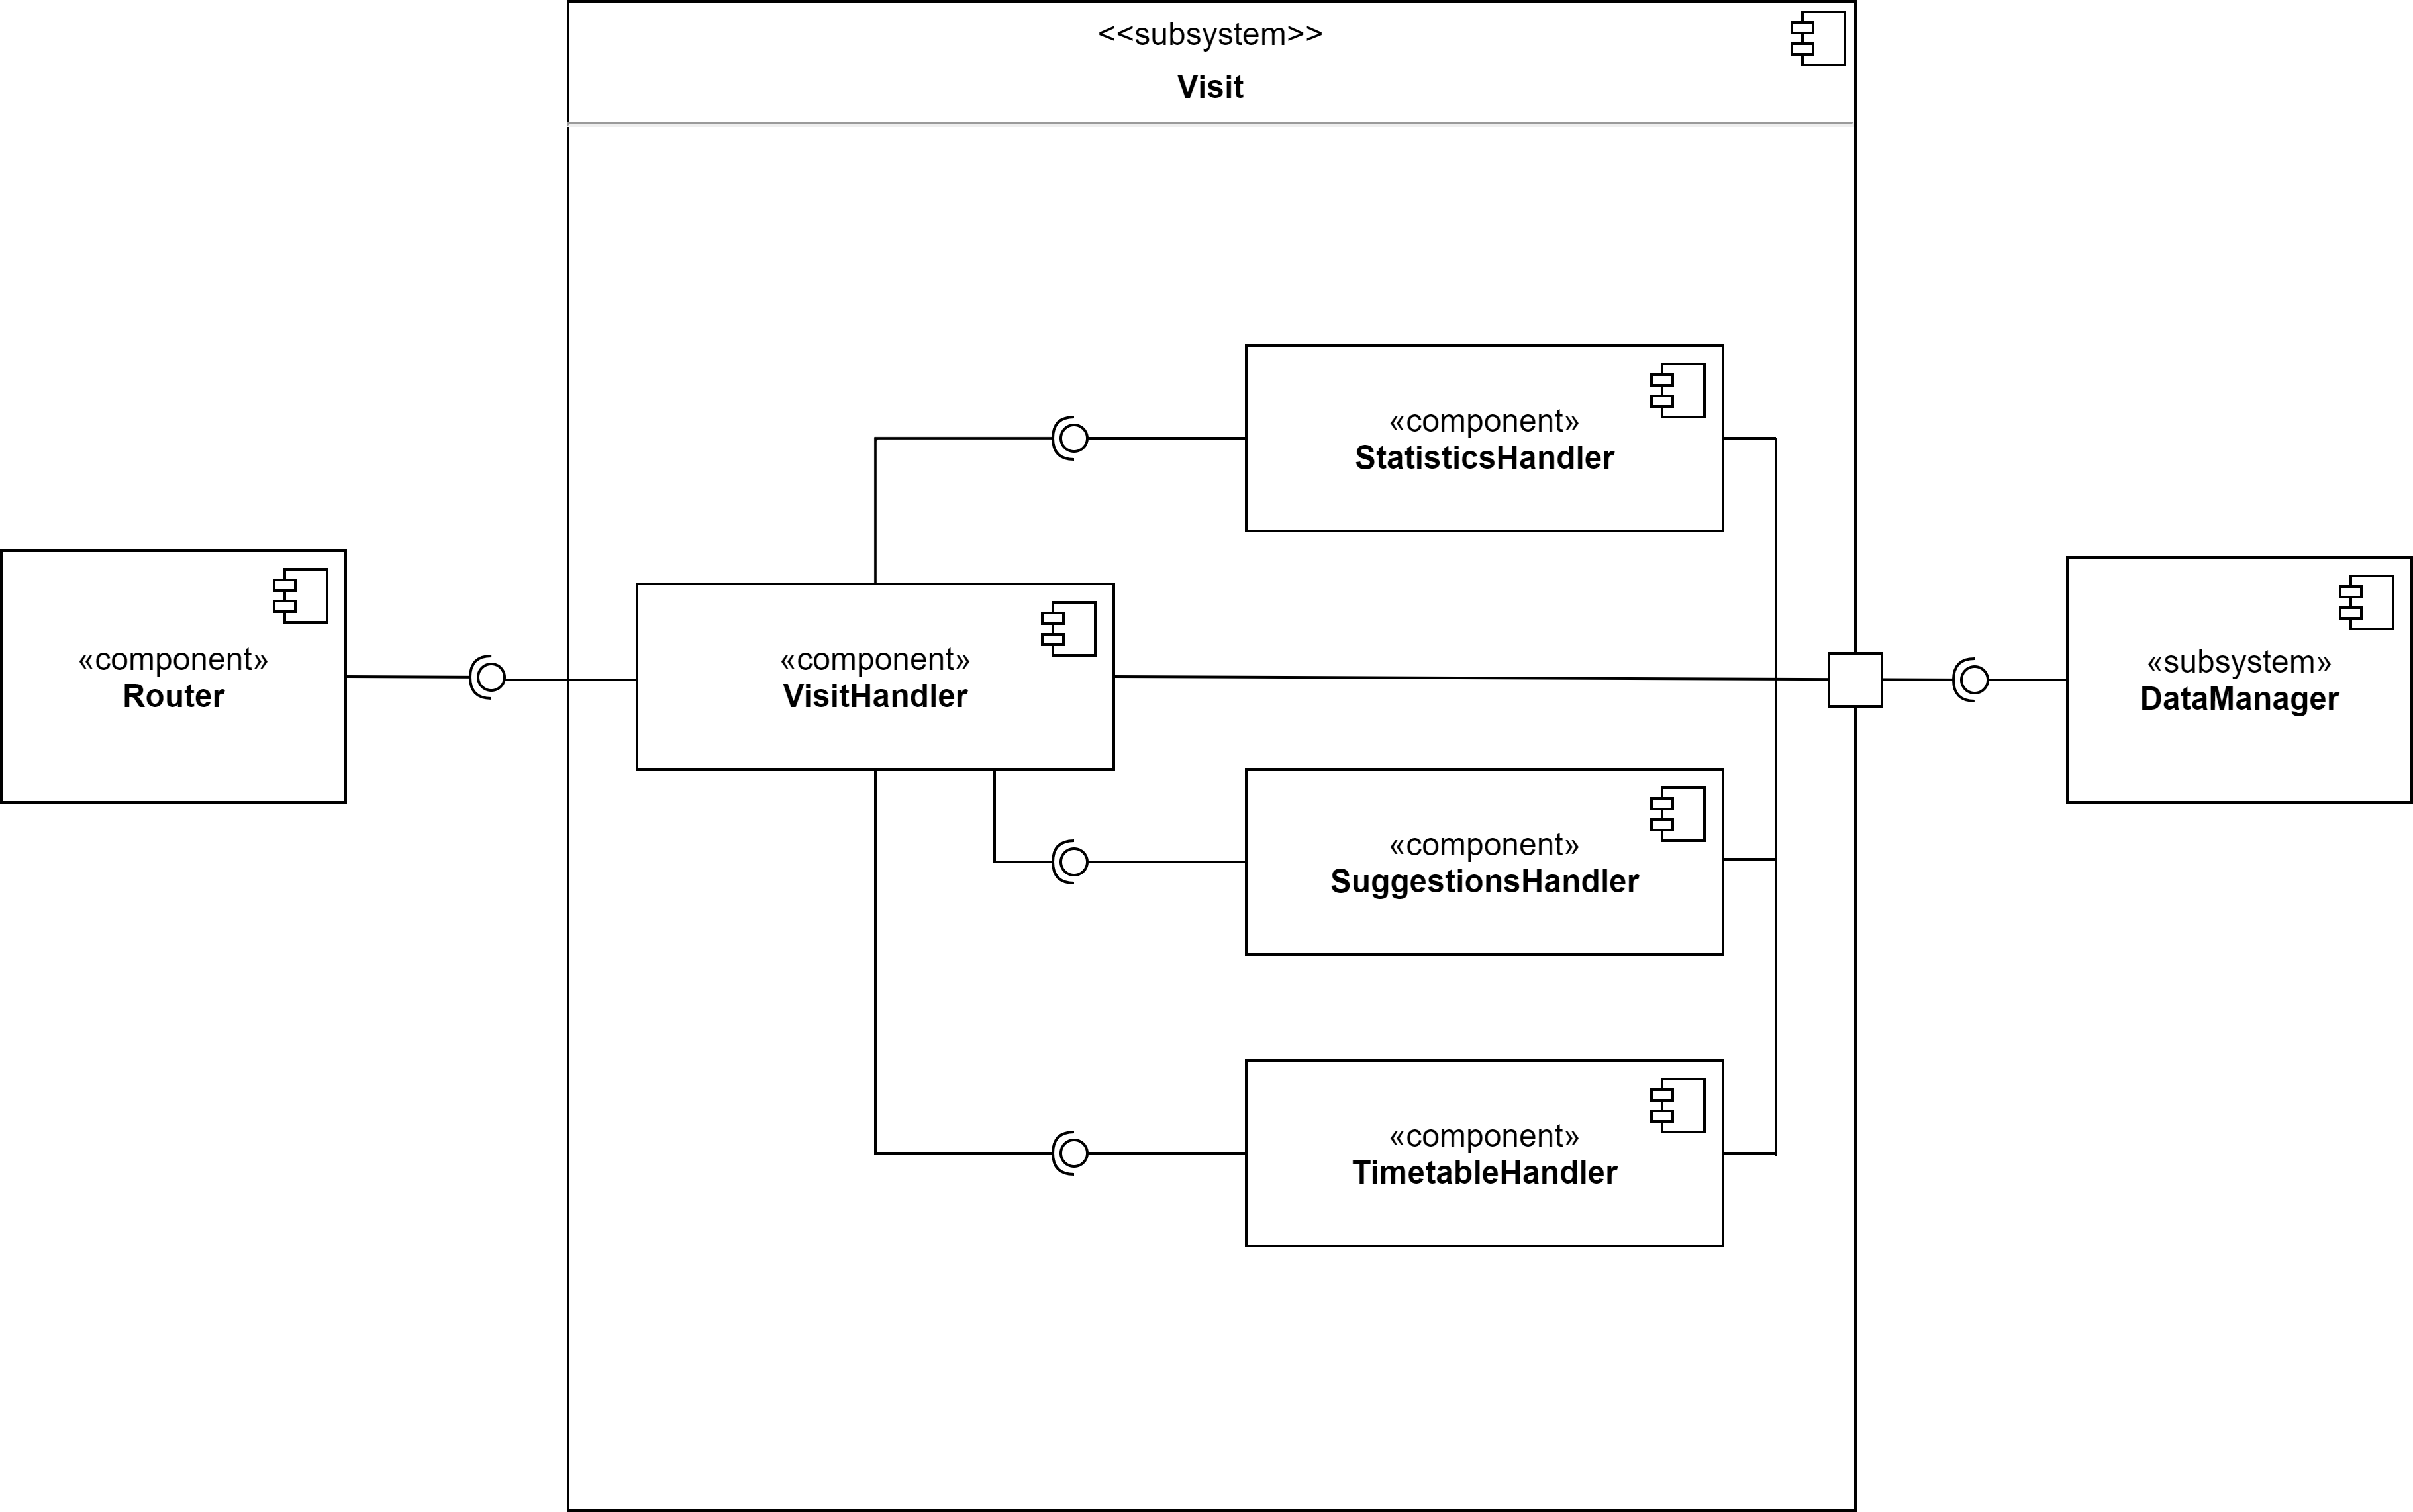
\includegraphics[scale=0.6]{VisitComponent}
		\caption{Visit subsystem}
		\label{fig:visitSubsystem}
	\end{figure}

	\begin{itemize}
		\item \textbf{VisitHandler} works as an "orchestrator". It handles the requests that comes from outside the subsystem and exploits the functionalities offered by the other components;
		\item \textbf{StatisticHandler} collects user statistics;
		\item \textbf{SuggestionsHandler} computes suggestions based on user preferences and timetable availability;
		\item \textbf{TimetableHandler} handles time-slots and computes their availability.
	\end{itemize}
	
				
	\newpage			
				
	\section{User Interface Design}
	This chapter aims to give a general idea of the user interface, both of the costumer mobile application and the store manager webapp. 
	This is done by means of mockups and UX diagrams.
		
		\subsection{Mockups}
		In the design process of the user interface the main guideline was the Requirement R2 (\textit{The user and manager applications are clear, intuitive and simple to use} - RASD). Therefore, the screen contains only the necessary components and the interaction with them is limited to a few of intuitive form and buttons.
		\\The presented mockups cover almost the totality of the screens you will find on the completed user interface. They show only the components needed to address the CLup goals, buttons such as "return to the previous screens" are not usually taken into account.
		
			\subsubsection{Mobile Application Mockups}
			\bigskip \bigskip \bigskip \bigskip
			\begin{figure}[h!] 
				\centering
				\subfloat[Sign-in screen]
				{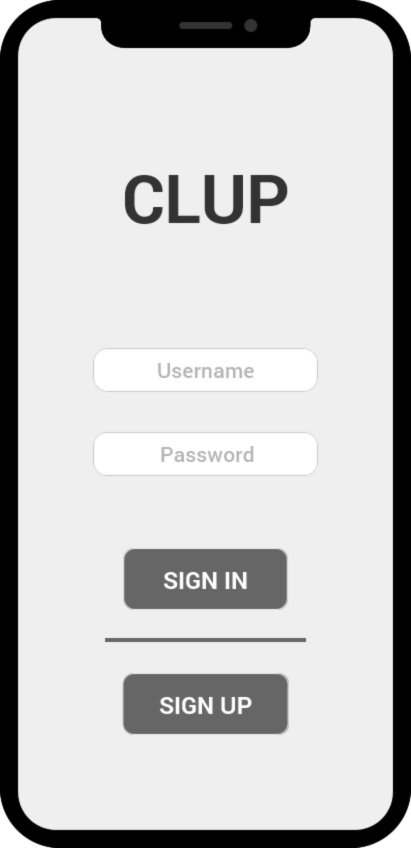
\includegraphics[width=.25\textwidth]{Mockups/signIn}}
				\qquad\qquad
				\subfloat[Sign-up screen]
				{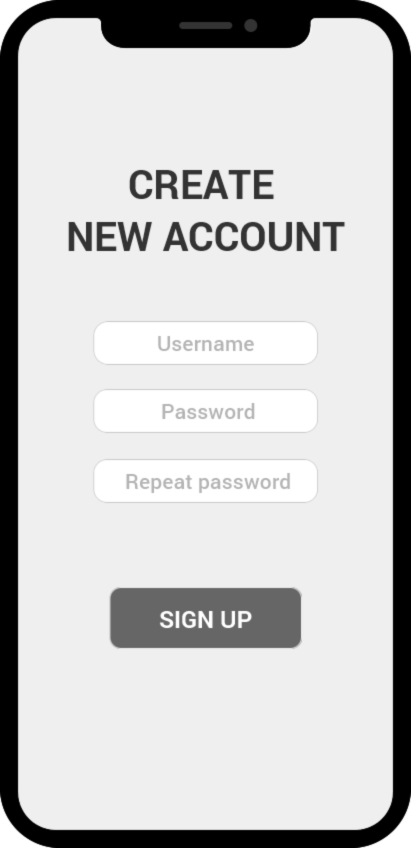
\includegraphics[width=.25\textwidth]{Mockups/signUp}}
				\qquad\qquad
				\subfloat[Store selection/booking check screen]
				{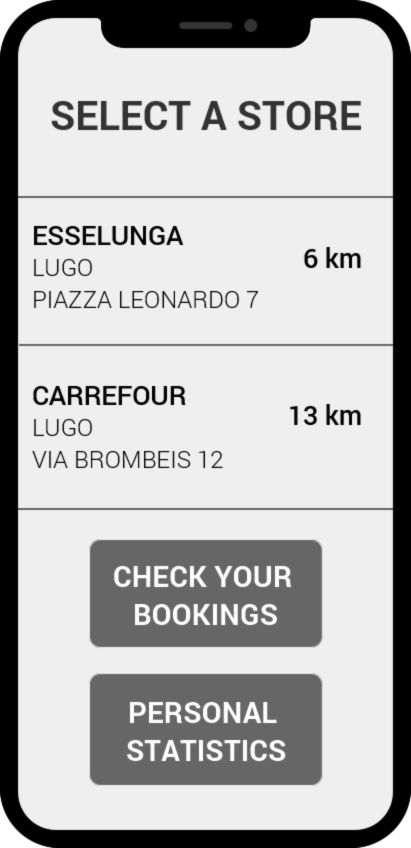
\includegraphics[width=.25\textwidth]{Mockups/selectStore}} 
			\end{figure}
		
			\newpage
			\begin{figure}[h!]\ContinuedFloat
				\centering
				\subfloat[Booking check screen]
				{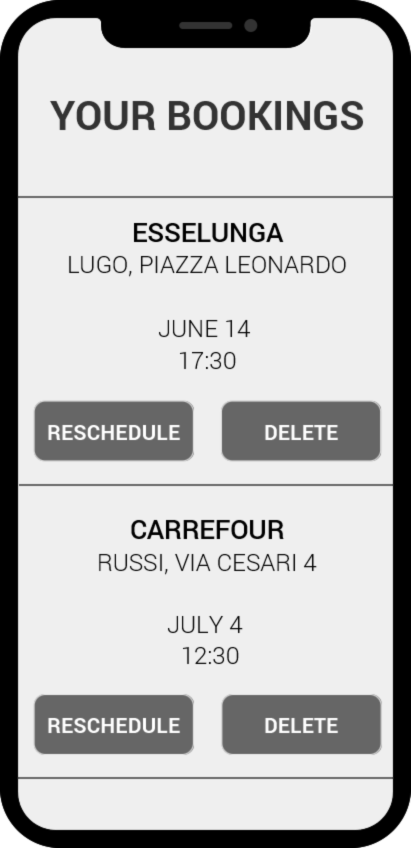
\includegraphics[width=.25\textwidth]{Mockups/bookingCheck}}
				\qquad\qquad
				\subfloat[Store available actions screen]
				{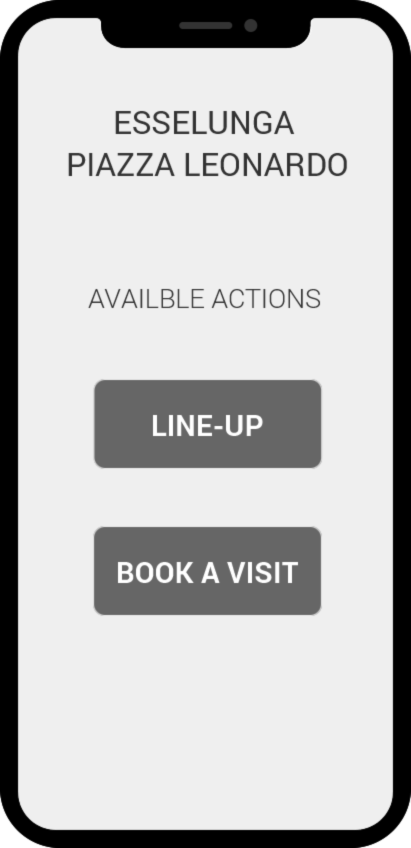
\includegraphics[width=.25\textwidth]{Mockups/storeAvailableActions}}
				\qquad\qquad
				\subfloat[Queue status screen]
				{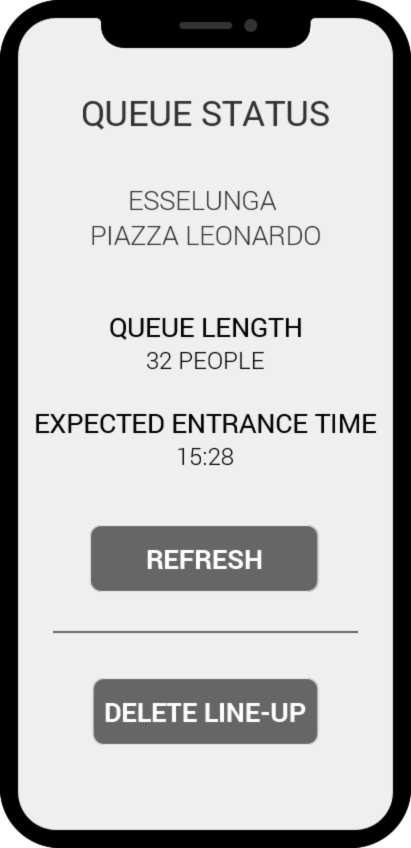
\includegraphics[width=.25\textwidth]{Mockups/queueStatus}} 
				
				\bigskip \bigskip \bigskip
				
				\subfloat[Book a visit screen]
				{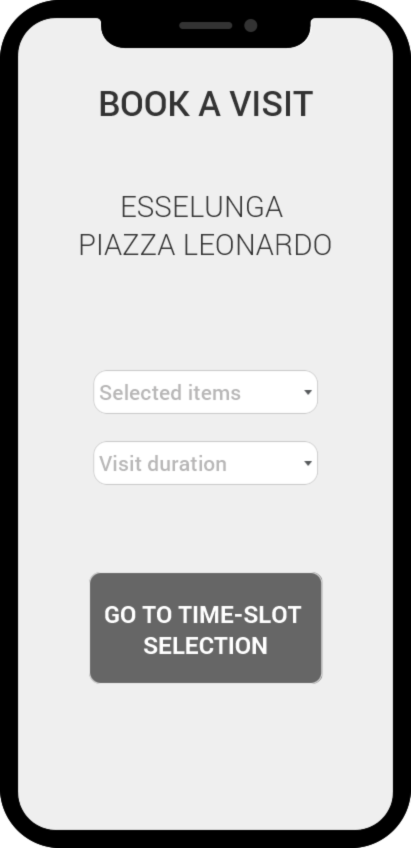
\includegraphics[width=.25\textwidth]{Mockups/bookVisit}}
				\qquad\qquad
				\subfloat[Time-slot selection screen]
				{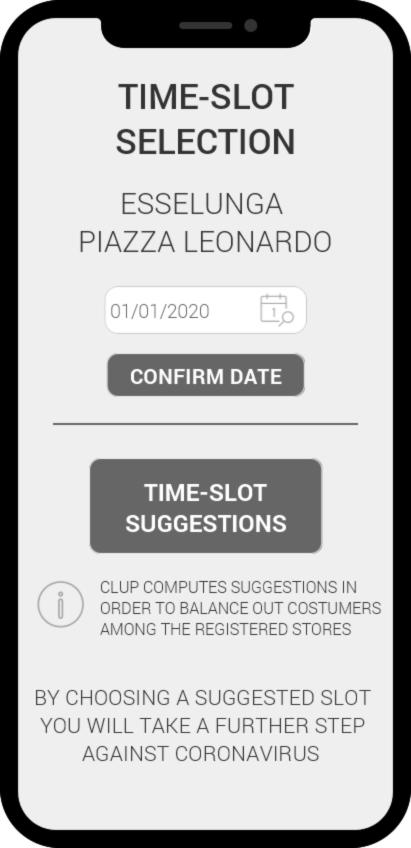
\includegraphics[width=.25\textwidth]{Mockups/timeSlotSelection}}
				\qquad\qquad
				\subfloat[CLup notification]
				{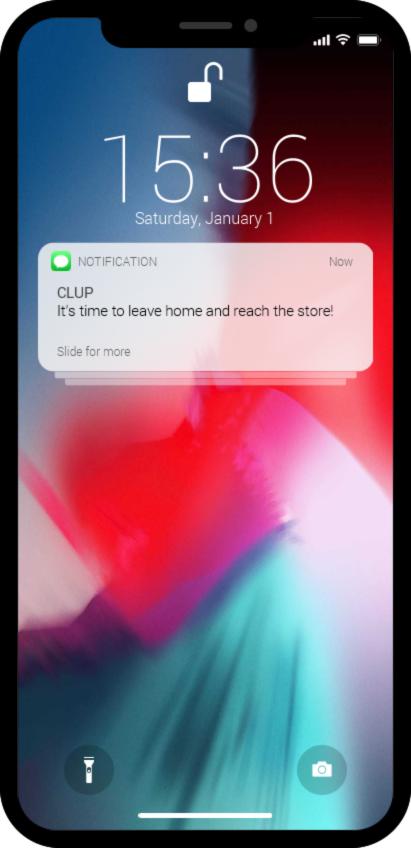
\includegraphics[width=.25\textwidth]{Mockups/notification}} 
			\end{figure}
		
			\newpage
			\subsubsection{WebApp Mockups}
			\bigskip
		
			\begin{figure}[H]
				\centering
				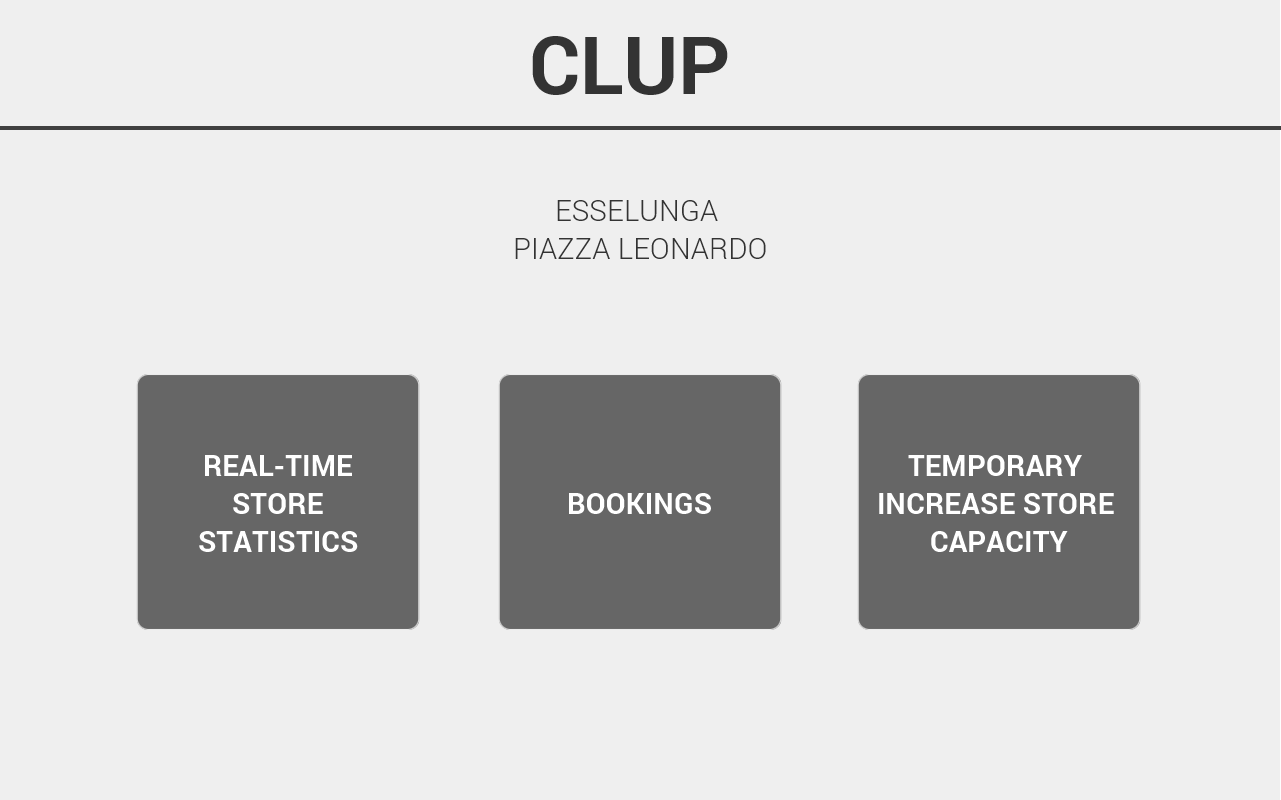
\includegraphics[scale=0.3]{Mockups/webAppHome}
				\caption{Home screen}
				\label{fig:homeScreen}
			\end{figure}
			\bigskip
			
			\begin{figure}[H]
				\centering
				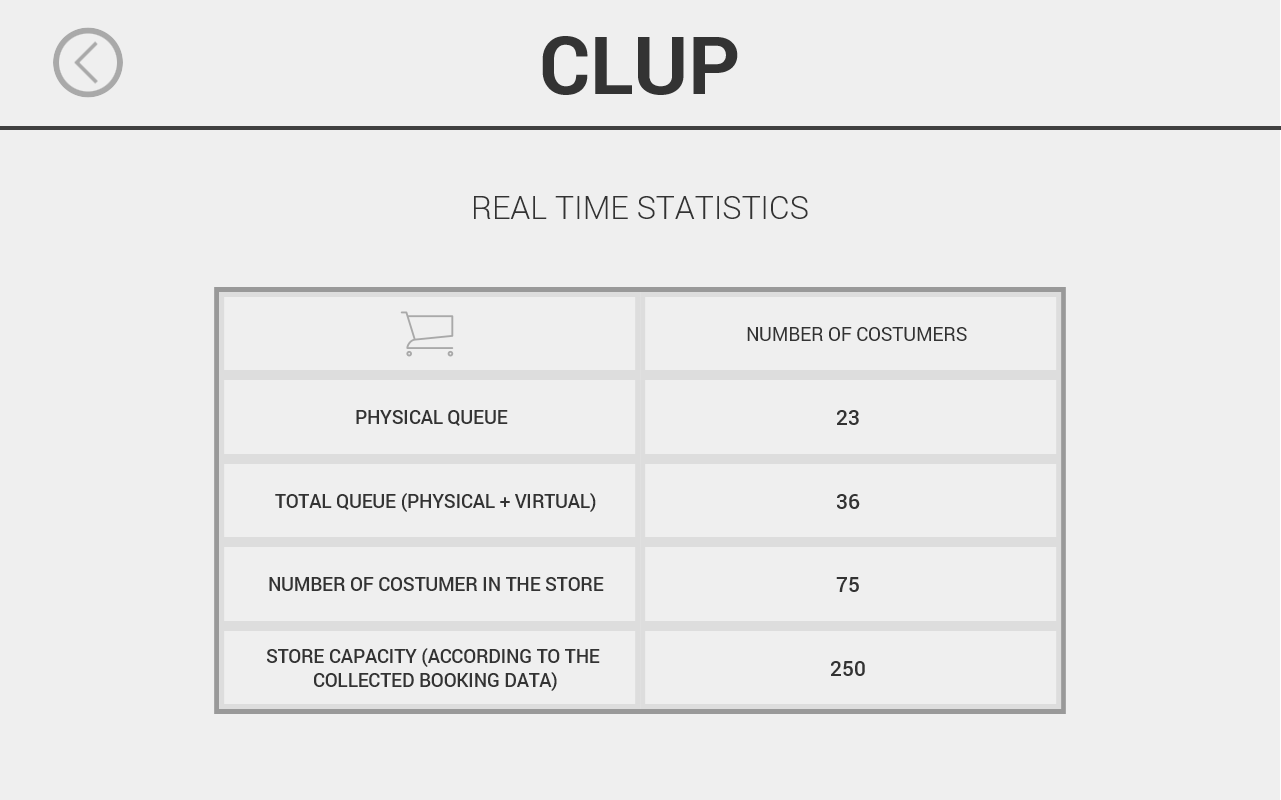
\includegraphics[scale=0.3]{Mockups/storeStatistics}
				\caption{Store statistics screen}
				\label{fig:Storestatisticsscreen}
			\end{figure}
		
			
			\begin{figure}[H]
				\centering
				\includegraphics[scale=0.3]{Mockups/storeBookings}
				\caption{Store bookings screen}
				\label{fig:ManagerHomeMockup}
			\end{figure}
		
		\newpage
		\subsection{UX diagrams}
		The chapter ends with two UX diagrams. They show the general flow of the screens giving more details on the user experience. "General" because some link between screens where omitted, like the "return" from a screen to the previous.
		
		\begin{figure}[H]
			
\includegraphics[scale=0.7]{UX diagrams/legend}
			\label{fig:MobileAppUXdiagram}
		\end{figure}
		\begin{figure}[H]
			\centering
			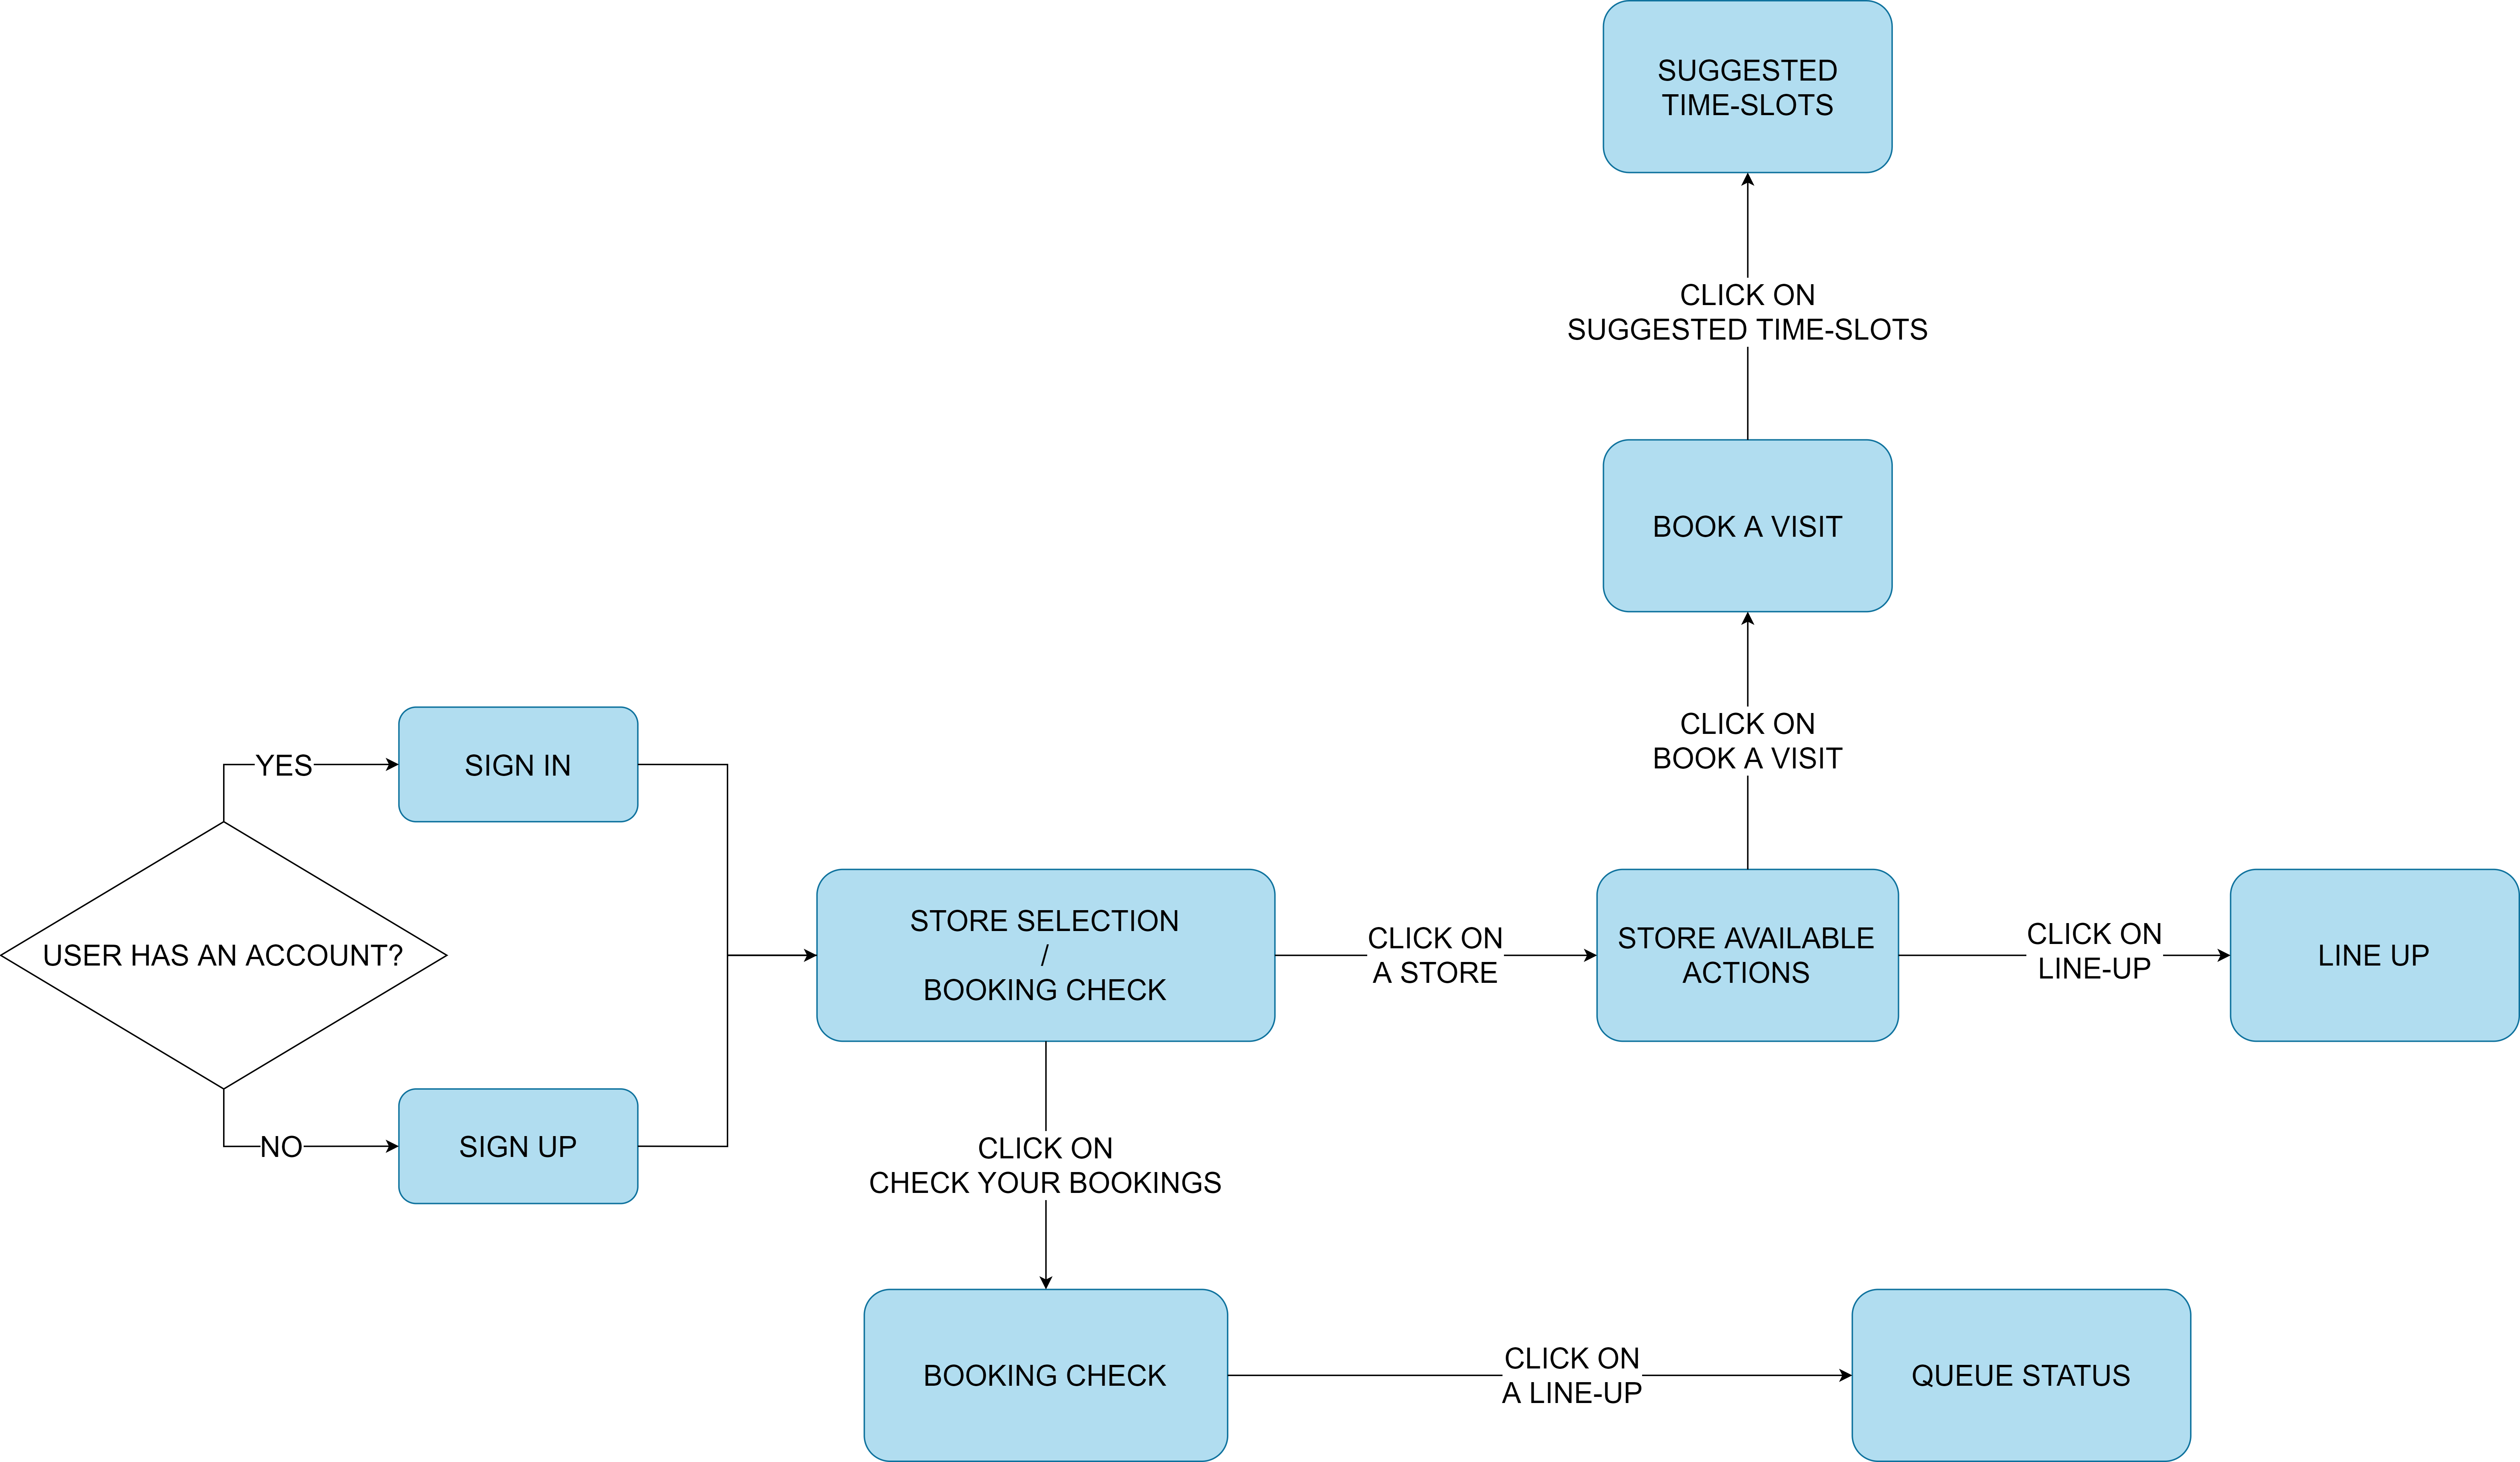
\includegraphics[scale=0.38]{UX diagrams/mobileApp}
			\caption{Mobile App UX diagram}
			\label{fig:MobileAppUXdiagram}
		\end{figure}
		\bigskip \bigskip \bigskip \bigskip
		\begin{figure}[H]
			\centering
			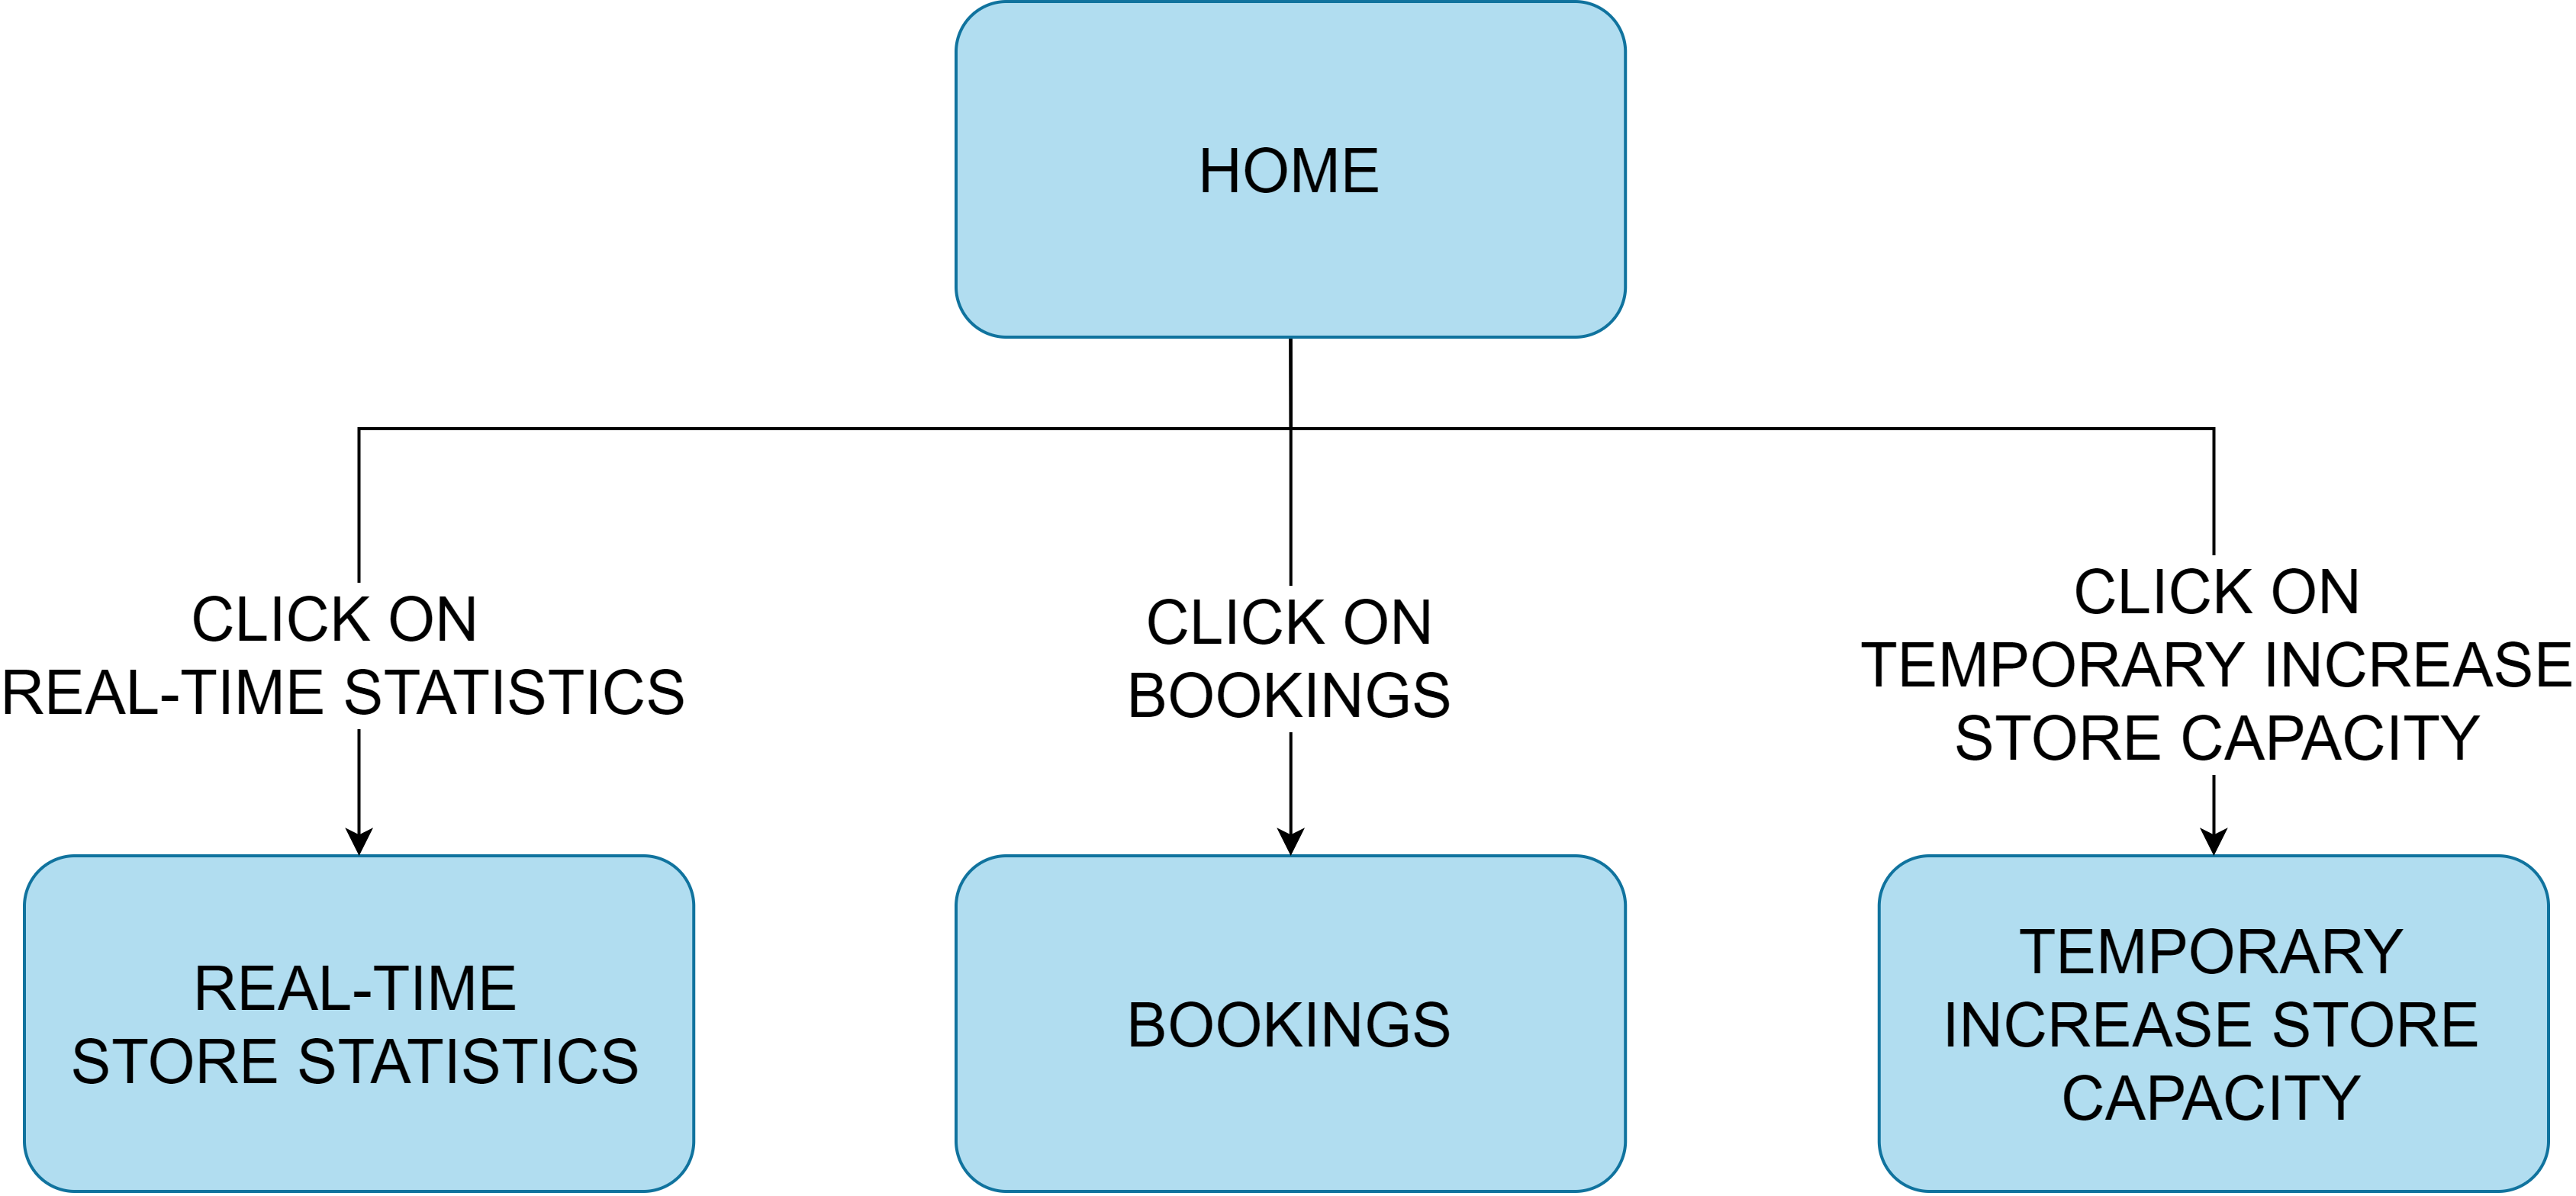
\includegraphics[scale=0.38]{UX diagrams/webAppHome}
			\caption{WebApp UX diagram}
			\label{fig:MobileAppUXdiagram}
		\end{figure}
			
		\newpage
		\section{Effort spent}
			
			\medskip
			\textbf{\large Antonio Ercolani:} \\ \newline
			\begin{tabular}{|l|c|}
				\hline
				Purpose and Document Structure &  \textbf{1h} \\ \hline
				\rowcolor[HTML]{DCDCDC} 
				User Interface Design & \textbf{8h} \\ \hline
				
			\end{tabular}
			\newline
			\newline
			
			\medskip
			\textbf{\large Vittorio Fabris:} \\ \newline
			\begin{tabular}{|l|c|}
				\hline
				Scope and organization of chapter 1&  \textbf{1h} \\ \hline
				\rowcolor[HTML]{DCDCDC} 
				 & \textbf{} \\ \hline
				
			\end{tabular}
	
			
			\section{References}	
			
			
	

				
\end{document}
